%! TeX program = xelatex
%! TEX TS-program = xelatex
\documentclass[12pt]{beamer}
\usepackage{fontspec}
\setsansfont{QTBookmann}
\usepackage{polyglossia}
\usepackage[dvipsnames]{xcolor}
\usepackage{dirtytalk}
\usepackage{graphicx}
\setdefaultlanguage{spanish}
\usepackage{multirow}
\usepackage[backend=biber]{biblatex}
%\usetheme{Copenhagen}
%%%%%%%%%%%%%%%%%%%%%%%%%%%%%%%%%%%%%%%%%%%%%%%%%%%%%%%%%%%%%%%%%%%%%%%%
%\definecolor{mypurple}{RGB}{044,040,028}                              %
%\setbeamercolor*{palette primary}{use=structure,fg=white,bg=mypurple} %
\definecolor{mypurple}{RGB}{195,084,023}                              %
\setbeamercolor*{palette primary}{use=structure,fg=white,bg=mypurple} %
\setbeamercolor{normal text}{fg=white}                                %
\setbeamercolor{titlelike}{fg=GreenYellow!80!White}
\setbeamercolor{bibliography entry author}{fg=Cyan!90!White}
\setbeamercolor{bibliography entry note}{fg=Maroon!20!White}
\setbeamercolor{bibliography item}{fg=Cyan!90!White}
\setbeamertemplate{navigation symbols}{}                              %
%%%%%%%%%%%%%%%%%%%%%%%%%%%%%%%%%%%%%%%%%%%%%%%%%%%%%%%%%%%%%%%%%%%%%%%%
\setbeamertemplate{background}{%
  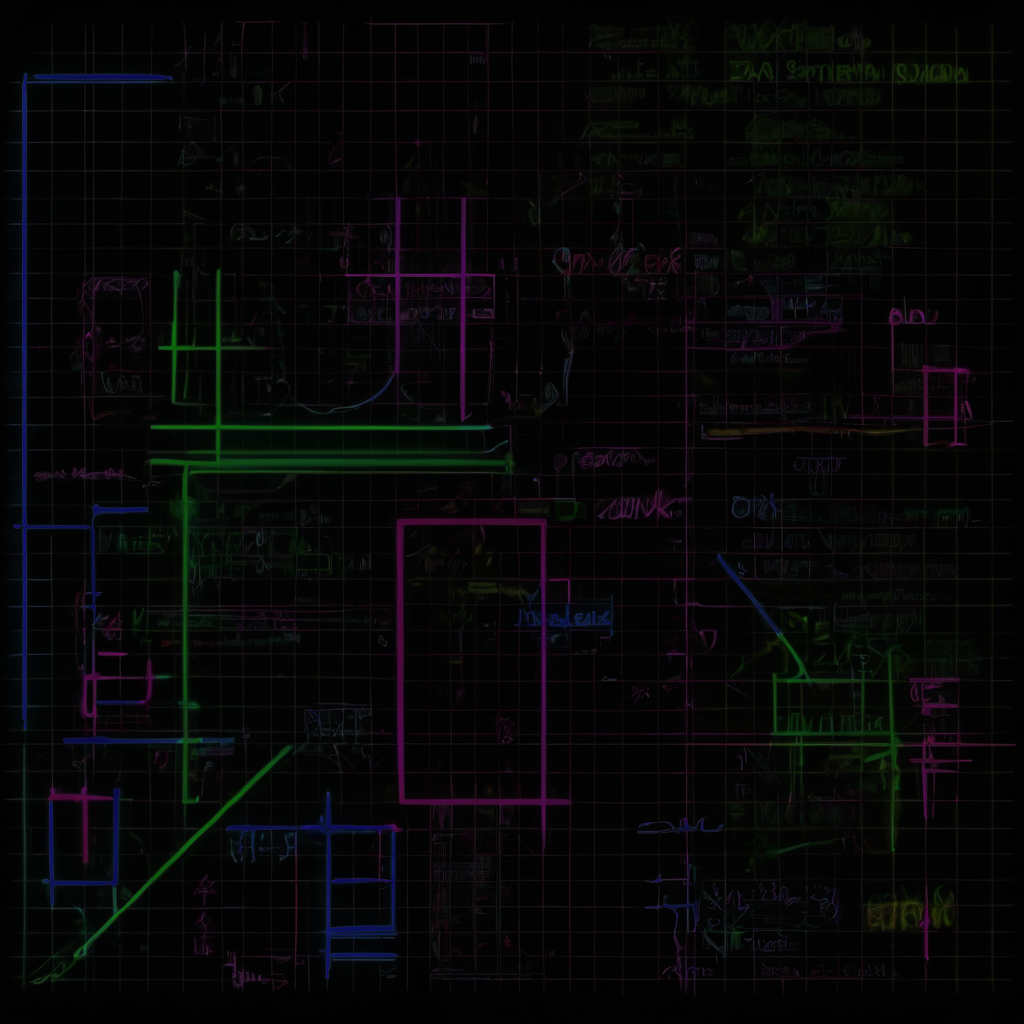
\includegraphics[width=\paperwidth]{fondo}
}
%%%%%%%%%%%%%%%%%%%%%%%%%%%%%%%%%%%%%%%%%%%%%%%%%%%%%%%%%%%%%%%%%%%%%%%%
\bibliography{bibliography}
\nocite{*}
\author{%
Brandon Marquez Salazar
}
\title{%
  Clasificador
}
%Duración no más de 15min
\begin{document}
  \frame{\titlepage}
  \begin{frame}
    {\Large Objetivo}

    El objetivo de este estudio es el reconocimiento de círculos y elipses a partir de
    métodos de optimización e inteligencia artificial.

  \end{frame}
  \begin{frame}
    {\Large Herramientas utilizadas}

    Se utilizaron algoritmos genéticos para la detección de tres puntos específicos,
    suficientes para la caracterización del círculo o elipse.
    \begin{center}
    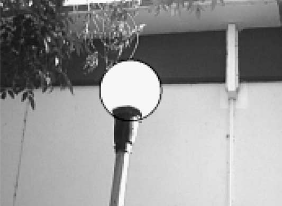
\includegraphics{example}
    \end{center}

  \end{frame}
  \begin{frame}
  {\Large Recurso}
  \printbibliography
  \end{frame}
\end{document}
